\chapter{Modelo Proposto Para Implementação da Experimentação Contínua}
\label{apdx:processo-novo}

Este apêndice apresenta o processo de desenvolvimento proposto neste trabalho para a implementação da experimentação no desenvolvimento do produto sendo avaliado, ilustrado nas Figuras \ref{fig:novo-process-a} e \ref{fig:novo-process-b}. O diagrama foi segmentado em duas partes para garantir a legibilidade de todas as fases, artefatos e atividades. As setas que conectam as figuras foram identificadas por letras em ordem alfabética, facilitando a compreensão do modelo como um todo.

\clearpage
\begin{landscape}
    \begin{figure}[p]
        \centering
        \caption{\textit{Modelo Proposto Para Implementação da Experimentação Contínua (Parte 1 de 2)}}
        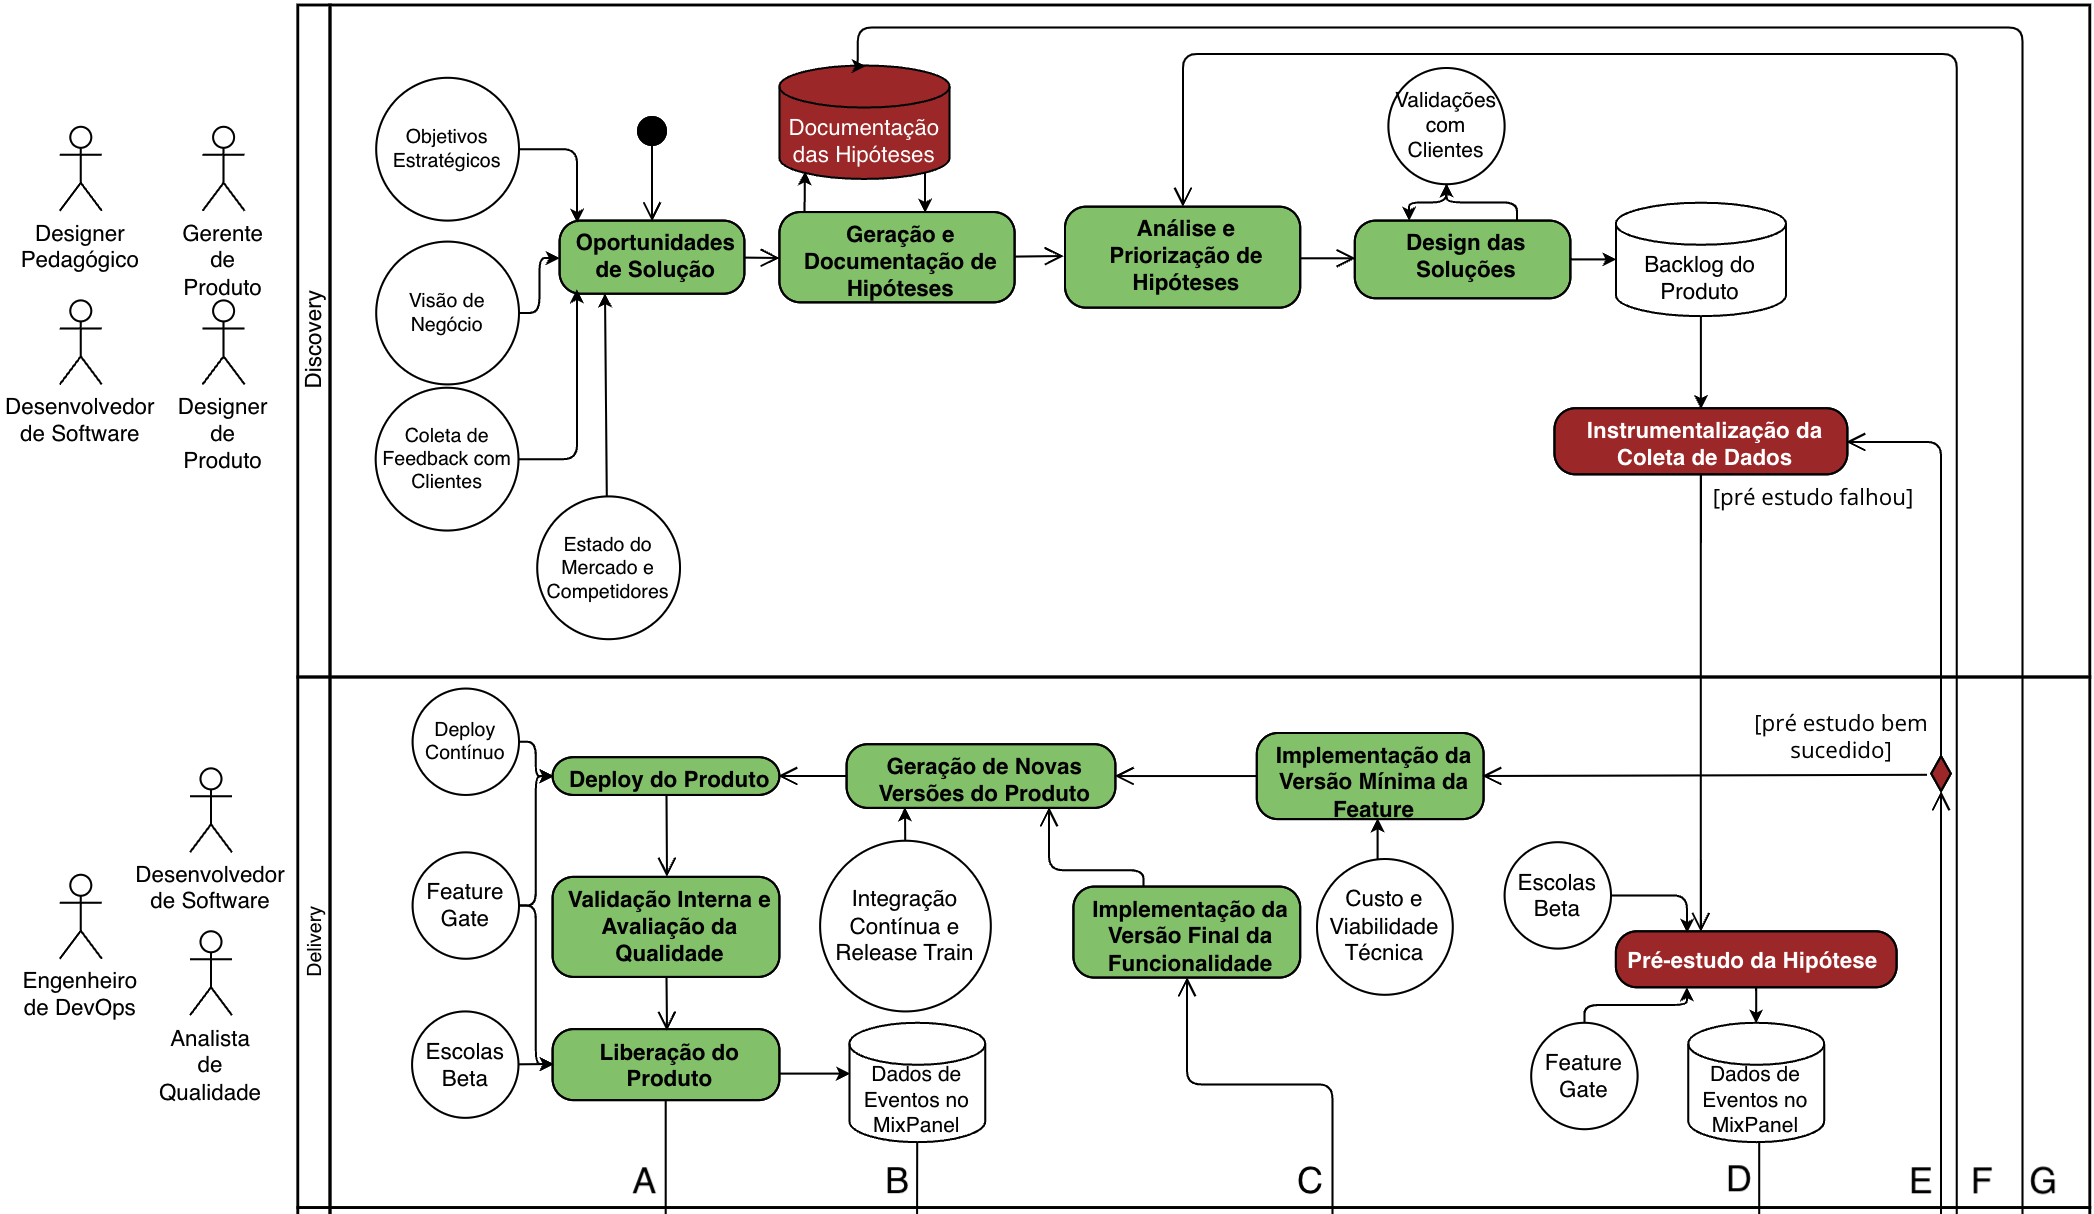
\includegraphics[width=1\linewidth]{figuras/processo_novo_a.png}
        \text{Fonte: Autor}
        \label{fig:novo-process-a}
    \end{figure}
\end{landscape}


\clearpage
\begin{landscape}
    \begin{figure}[p]
        \centering
        \caption{\textit{Modelo Proposto Para Implementação da Experimentação Contínua (Parte 2 de 2)}}
        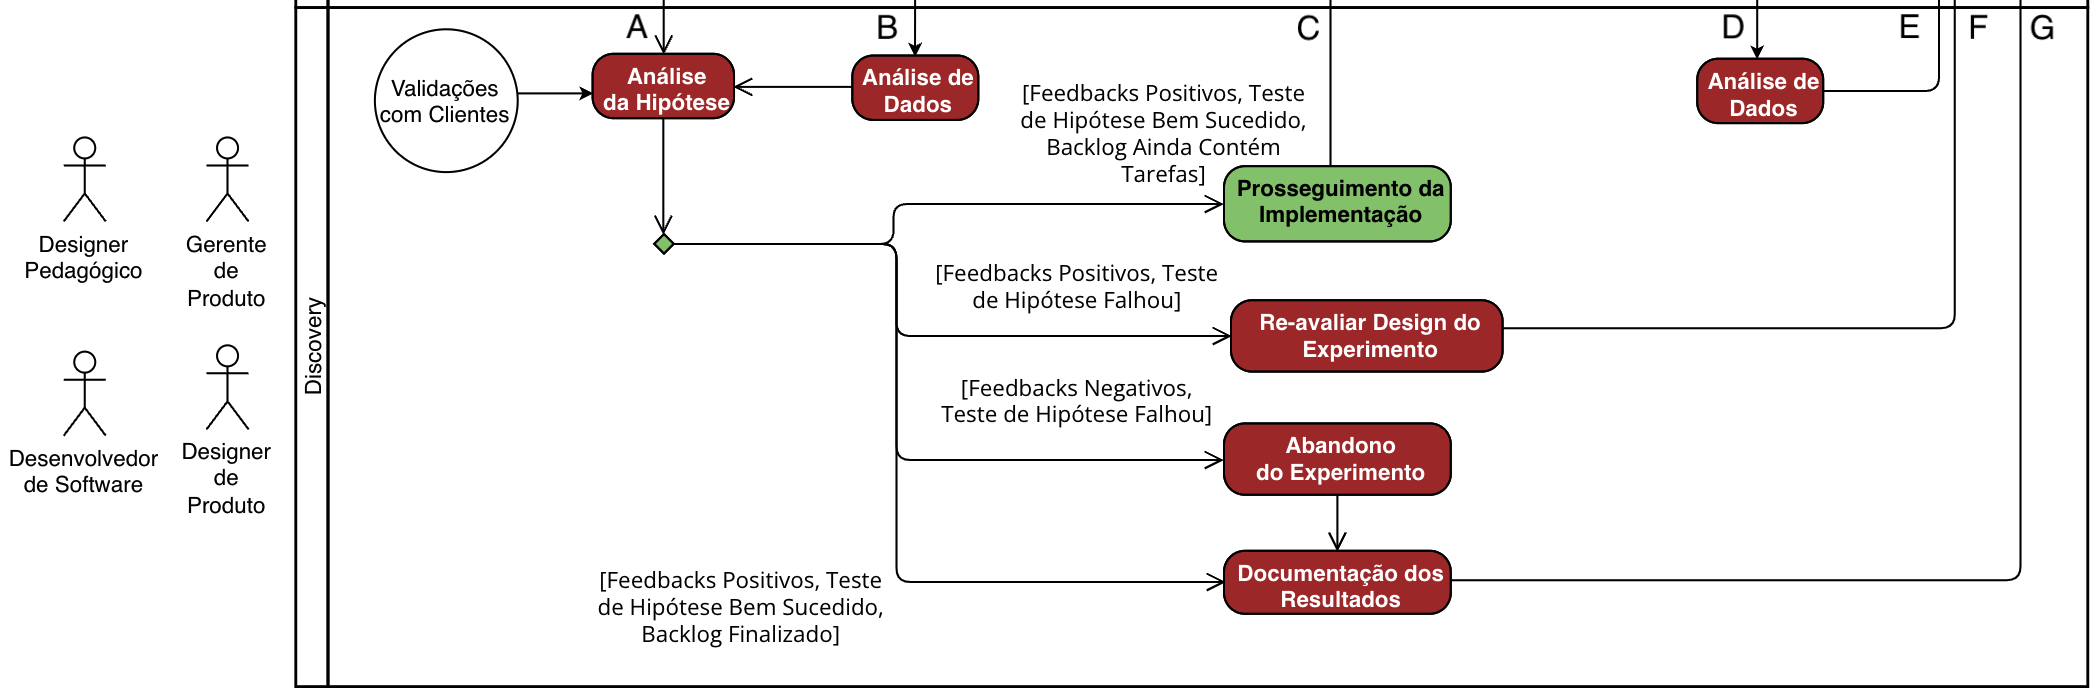
\includegraphics[width=1\linewidth]{figuras/processo_novo_b.png}
        \text{Fonte: Autor}
        \label{fig:novo-process-b}
    \end{figure}
\end{landscape}


